% arara: pdflatex
% arara: pdflatex
% arara: pdflatex

% options:
% thesis=B bachelor's thesis
% thesis=M master's thesis
% czech thesis in Czech language
% slovak thesis in Slovak language
% english thesis in English language
% hidelinks remove colour boxes around hyperlinks

\documentclass[thesis=B,czech]{FITthesis}[2019/12/23]

\usepackage[latin2]{inputenc} % LaTeX source encoded as ISO-8859-2

% \usepackage{amsmath} %advanced maths
% \usepackage{amssymb} %additional math symbols

\usepackage{dirtree} %directory tree visualisation

% % list of acronyms
% \usepackage[acronym,nonumberlist,toc,numberedsection=autolabel]{glossaries}
% \iflanguage{czech}{\renewcommand*{\acronymname}{Seznam pou{\v z}it{\' y}ch zkratek}}{}
% \makeglossaries

\newcommand{\tg}{\mathop{\mathrm{tg}}} %cesky tangens
\newcommand{\cotg}{\mathop{\mathrm{cotg}}} %cesky cotangens

% % % % % % % % % % % % % % % % % % % % % % % % % % % % % % 
% ODTUD DAL VSE ZMENTE
% % % % % % % % % % % % % % % % % % % % % % % % % % % % % % 

\department{Katedra \ldots (DOPLÒTE)}
\title{Doplòte název práce}
\authorGN{Doplòte Va¹e køestní jméno/jména} %(køestní) jméno (jména) autora
\authorFN{Doplòte Va¹e pøíjmení} %pøíjmení autora
\authorWithDegrees{Doplòte Va¹e jméno a tituly} %jméno autora vèetnì souèasných akademických titulù
\author{Jan Nový} %jméno autora bez akademických titulù
\supervisor{Doplòte jméno vedoucího práce}
\acknowledgements{Doplòte, máte-li komu a za co dìkovat. V~opaèném pøípadì úplnì odstraòte tento pøíkaz.}
\abstractCS{V~nìkolika vìtách shròte obsah a pøínos této práce v~èe¹tinì. Po pøeètení abstraktu by se ètenáø mìl mít ètenáø dost informací pro rozhodnutí, zda chce Va¹i práci èíst.}
\abstractEN{Sem doplòte ekvivalent abstraktu Va¹í práce v~angliètinì.}
\placeForDeclarationOfAuthenticity{V~Praze}
\declarationOfAuthenticityOption{4} %volba Prohlá¹ení (èíslo 1-6)
\keywordsCS{Nahraïte seznamem klíèových slov v èe¹tinì oddìlených èárkou.}
\keywordsEN{Nahraïte seznamem klíèových slov v angliètinì oddìlených èárkou.}
% \website{http://site.example/thesis} %volitelná URL práce, objeví se v tirá¾i - úplnì odstraòte, nemáte-li URL práce

\begin{document}

% \newacronym{CVUT}{{\v C}VUT}{{\v C}esk{\' e} vysok{\' e} u{\v c}en{\' i} technick{\' e} v Praze}
% \newacronym{FIT}{FIT}{Fakulta informa{\v c}n{\' i}ch technologi{\' i}}

\begin{introduction}
	%sem napi¹te úvod Va¹í práce
\end{introduction}

\chapter{Cíl práce}

\chapter{Analýza a návrh}

\chapter{Realizace}

\begin{conclusion}
	%sem napi¹te závìr Va¹í práce
\end{conclusion}

\bibliographystyle{csn690}
\bibliography{mybibliographyfile}

\appendix

\chapter{Seznam pou¾itých zkratek}
% \printglossaries
\begin{description}
	\item[GUI] Graphical user interface
	\item[XML] Extensible markup language
\end{description}


% % % % % % % % % % % % % % % % % % % % % % % % % % % % 
% % Tuto kapitolu z výsledné práce ODSTRAÒTE.
% % % % % % % % % % % % % % % % % % % % % % % % % % % % 
% 
% \chapter{Návod k~pou¾ití této ¹ablony}
% 
% Tento dokument slou¾í jako základ pro napsání závìreèné práce na Fakultì informaèních technologií ÈVUT v~Praze.
% 
% \section{Výbìr základu}
% 
% Vyberte si ¹ablonu podle druhu práce (bakaláøská, diplomová), jazyka (èe¹tina, angliètina) a kódování (ASCII, \mbox{UTF-8}, \mbox{ISO-8859-2} neboli latin2 a nebo \mbox{Windows-1250}). 
% 
% V~èeské variantì naleznete ¹ablony v~souborech pojmenovaných ve formátu práce\_kódování.tex. Typ mù¾e být:
% \begin{description}
% 	\item[BP] bakaláøská práce,
% 	\item[DP] diplomová (magisterská) práce.
% \end{description}
% Kódování, ve kterém chcete psát, mù¾e být:
% \begin{description}
% 	\item[UTF-8] kódování Unicode,
% 	\item[ISO-8859-2] latin2,
% 	\item[Windows-1250] znaková sada 1250 Windows.
% \end{description}
% V~pøípadì nejistoty ohlednì kódování doporuèujeme následující postup:
% \begin{enumerate}
% 	\item Otevøete ¹ablony pro kódování UTF-8 v~editoru prostého textu, který chcete pro psaní práce pou¾ít -- pokud mù¾ete texty s~diakritikou normálnì pøeèíst, pou¾ijte tuto ¹ablonu.
% 	\item V~opaèném pøípadì postupujte dále podle toho, jaký operaèní systém pou¾íváte:
% 	\begin{itemize}
% 		\item v~pøípadì Windows pou¾ijte ¹ablonu pro kódování \mbox{Windows-1250},
% 		\item jinak zkuste pou¾ít ¹ablonu pro kódování \mbox{ISO-8859-2}.
% 	\end{itemize}
% \end{enumerate}
% 
% 
% V~anglické variantì jsou ¹ablony pojmenované podle typu práce, mo¾nosti jsou:
% \begin{description}
% 	\item[bachelors] bakaláøská práce,
% 	\item[masters] diplomová (magisterská) práce.
% \end{description}
% 
% \section{Pou¾ití ¹ablony}
% 
% ©ablona je urèena pro zpracování systémem \LaTeXe{}. Text je mo¾né psát v~textovém editoru jako prostý text, lze v¹ak také vyu¾ít specializovaný editor pro \LaTeX{}, napø. Kile.
% 
% Pro získání tisknutelného výstupu z~takto vytvoøeného souboru pou¾ijte pøíkaz \verb|pdflatex|, kterému pøedáte cestu k~souboru jako parametr. Vhodný editor pro \LaTeX{} toto udìlá za Vás. \verb|pdfcslatex| ani \verb|cslatex| \emph{nebudou} s~tìmito ¹ablonami fungovat.
% 
% Více informací o~pou¾ití systému \LaTeX{} najdete napø. v~\cite{wikilatex}.
% 
% \subsection{Typografie}
% 
% Pøi psaní dodr¾ujte typografické konvence zvoleného jazyka. Èeské \uv{uvozovky} zapisujte pou¾itím pøíkazu \verb|\uv|, kterému v~parametru pøedáte text, jen¾ má být v~uvozovkách. Anglické otevírací uvozovky se v~\LaTeX{}u zadávají jako dva zpìtné apostrofy, uzavírací uvozovky jako dva apostrofy. Èasto chybnì uvádìný symbol "{} (palce) nemá s~uvozovkami nic spoleèného.
% 
% Dále je tøeba zabránit zalomení øádky mezi nìkterými slovy, v~èe¹tinì napø. za jednopísmennými pøedlo¾kami a spojkami (vyjma \uv{a}). To docílíte vlo¾ením pru¾né nezalomitelné mezery -- znakem \texttt{\textasciitilde}. V~tomto pøípadì to není tøeba dìlat ruènì, lze pou¾ít program \verb|vlna|.
% 
% Více o~typografii viz \cite{kobltypo}.
% 
% \subsection{Obrázky}
% 
% Pro umo¾nìní vkládání obrázkù je vhodné pou¾ít balíèek \verb|graphicx|, samotné vlo¾ení se provede pøíkazem \verb|\includegraphics|. Takto je mo¾né vkládat obrázky ve formátu PDF, PNG a JPEG jestli¾e pou¾íváte pdf\LaTeX{} nebo ve formátu EPS jestli¾e pou¾íváte \LaTeX{}. Doporuèujeme preferovat vektorové obrázky pøed rastrovými (vyjma fotografií).
% 
% \subsubsection{Získání vhodného formátu}
% 
% Pro získání vektorových formátù PDF nebo EPS z~jiných lze pou¾ít nìkterý z~vektorových grafických editorù. Pro pøevod rastrového obrázku na vektorový lze pou¾ít rasterizaci, kterou mnohé editory zvládají (napø. Inkscape). Pro konverze lze pou¾ít té¾ nástroje pro dávkové zpracování bì¾nì dodávané s~\LaTeX{}em, napø. \verb|epstopdf|.
% 
% \subsubsection{Plovoucí prostøedí}
% 
% Pøíkazem \verb|\includegraphics| lze obrázky vkládat pøímo, doporuèujeme v¹ak pou¾ít plovoucí prostøedí, konkrétnì \verb|figure|. Napøíklad obrázek \ref{fig:float} byl vlo¾en tímto zpùsobem. Vùbec pøitom nevadí, kdy¾ je obrázek umístìn jinde, ne¾ bylo pùvodnì zamý¹leno -- je tomu tak hlavnì kvùli dodr¾ení typografických konvencí. Namísto vynucování konkrétní pozice obrázku doporuèujeme pou¾ívat odkazování z~textu (dvojice pøíkazù \verb|\label| a \verb|\ref|).
% 
% \begin{figure}\centering
% 	
\includegraphics[width=0.5\textwidth, angle=30]{cvut-logo-bw}
% 	\caption[Pøíklad obrázku]{Ukázkový obrázek v~plovoucím prostøedí}\label{fig:float}
% \end{figure}
% 
% \subsubsection{Verze obrázkù}
% 
% % Gnuplot BW i barevnì
% Mù¾e se hodit mít více verzí stejného obrázku, napø. pro barevný èi èernobílý tisk a nebo pro prezentaci. S~pomocí nìkterých nástrojù na generování grafiky je to snadné.
% 
% Máte-li napøíklad graf vytvoøený v programu Gnuplot, mù¾ete jeho èernobílou variantu (viz obr. \ref{fig:gnuplot-bw}) vytvoøit parametrem \verb|monochrome dashed| pøíkazu \verb|set term|. Barevnou variantu (viz obr. \ref{fig:gnuplot-col}) vhodnou na prezentace lze vytvoøit parametrem \verb|colour solid|.
% 
% \begin{figure}\centering
% 	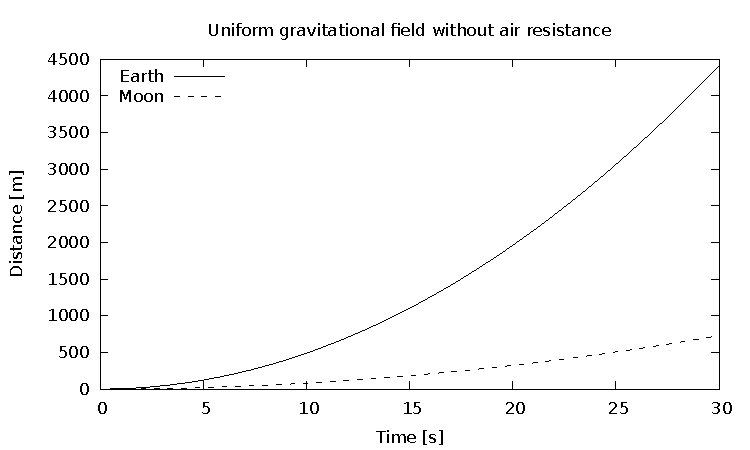
\includegraphics{gnuplot-bw}
% 	\caption{Èernobílá varianta obrázku generovaného programem Gnuplot}\label{fig:gnuplot-bw}
% \end{figure}
% 
% \begin{figure}\centering
% 	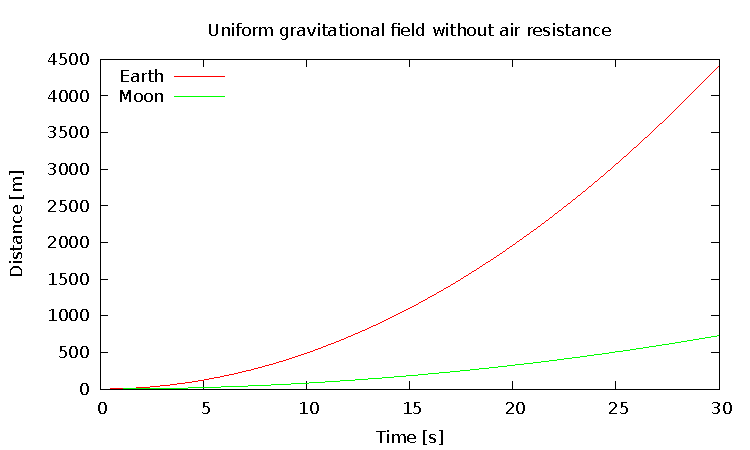
\includegraphics{gnuplot-col}
% 	\caption{Barevná varianta obrázku generovaného programem Gnuplot}\label{fig:gnuplot-col}
% \end{figure}
% 
% 
% \subsection{Tabulky}
% 
% Tabulky lze zadávat rùznì, napø. v~prostøedí \verb|tabular|, av¹ak pro jejich vkládání platí to samé, co pro obrázky -- pou¾ijte plovoucí prostøedí, v~tomto pøípadì \verb|table|. Napøíklad tabulka \ref{tab:matematika} byla vlo¾ena tímto zpùsobem.
% 
% \begin{table}\centering
% 	\caption[Pøíklad tabulky]{Zadávání matematiky}\label{tab:matematika}
% 	\begin{tabular}{|l|l|c|c|}\hline
% 		Typ		& Prostøedí		& \LaTeX{}ovská zkratka	& \TeX{}ovská zkratka	\tabularnewline \hline \hline
% 		Text		& \verb|math|		& \verb|\(...\)|	& \verb|$...$|		\tabularnewline \hline
% 		Displayed	& \verb|displaymath|	& \verb|\[...\]|	& \verb|$$...$$|	\tabularnewline \hline
% 	\end{tabular}
% \end{table}
% 
% % % % % % % % % % % % % % % % % % % % % % % % % % % % 

\chapter{Obsah pøilo¾eného CD}

%upravte podle skutecnosti

\begin{figure}
	\dirtree{%
		.1 readme.txt\DTcomment{struèný popis obsahu CD}.
		.1 exe\DTcomment{adresáø se spustitelnou formou implementace}.
		.1 src.
		.2 impl\DTcomment{zdrojové kódy implementace}.
		.2 thesis\DTcomment{zdrojová forma práce ve formátu \LaTeX{}}.
		.1 text\DTcomment{text práce}.
		.2 thesis.pdf\DTcomment{text práce ve formátu PDF}.
		.2 thesis.ps\DTcomment{text práce ve formátu PS}.
	}
\end{figure}

\end{document}
